% !TEX encoding = UTF-8 Unicode

\chapter{Konstruktion der \boldmath{$\alpha$}-Shape}

Im vorherigen Kapitel wurde gezeigt, dass die $\alpha$-Shape ein Subgraph des Delaunay-Graphen ist und es wurden die Shape-Spektren sowie die Shape-Schwellen definiert.

Hier wird nun ein Algorithmus gezeigt, welcher aus Minimum- und Maximum-Voronoi-Diagrammen einer Punktmenge $S$ die Shape-Spektren der Delaunay-Graphen von $S$ sowie die Shape-Schwellen von $S$ bestimmt. Anschließend wird ein Algorithmus gezeigt, welcher, mit $\alpha$ und den Shape-Spektren der Delaunay-Graphen von $S$ als Eingabe, die $\alpha$-Shape von $S$ bestimmt. Es werden weitere Algorithmen gezeigt, mit welchen, unter Ausnutzung des Shape-Spektrums, verschiedene interessante geometrische Eigenschaften von $S$ bestimmt werden können.

Zuerst wird kurz auf Algorithmen zur Erstellung von Voronoi-Diagrammen und auf die doppelt verkettete Kantenliste eingegangen. Dies ist der abstrakte Datentyp, in welchem die Voronoi-Diagramme für die Bestimmung von Shape-Spektren abgespeichert werden.

\section{Algorithmen zur Erstellung von Voronoi-Diagrammen}

Da die Erstellung von Voronoi-Diagrammen nicht das zentrale Thema dieser Arbeit ist, wird auf die implementierten Algorithmen und Datenstrukturen nur kurz eingegangen.

\subsection*{Fortunes Algorithmus}

In \autocite{deBerg2010} wird Fortunes Algorithmus zur Bestimmung eines \- Minimum-Voronoi-Diagramms beschrieben. Dabei handelt es sich um einen \- Plane-Sweep-Algo\-rithmus. Für die folgende Betrachtung wird die Sweep-Line von oben nach unten über die Ebene bewegt.

Die Bereiche oberhalb der Sweep-Line, welche sich im Voronoi-Diagramm nicht mehr ändern, werden durch sich schneidende Parabelbögen, der sogenannten Küstenlinie, bestimmt. Die Küstenlinie wird in einem AVL-Baum, wie er in \autocite{Gueting2004} beschrieben wird, gespeichert. Die innere Knoten des Baums sind die Schnittpunkte und seine Blätter sind die Parabelbögen. Der Verlauf der Schnittpunkte der Parabelbögen bestimmt den Verlauf der Kanten im Voronoi-Diagramm. Verschwindet ein Parabelbogen, so ist an dieser Stelle ein Knoten.

\begin{figure}[htbp]
	\centering
	\subfloat[Küstenlinie\label{fig:beachline}]
		{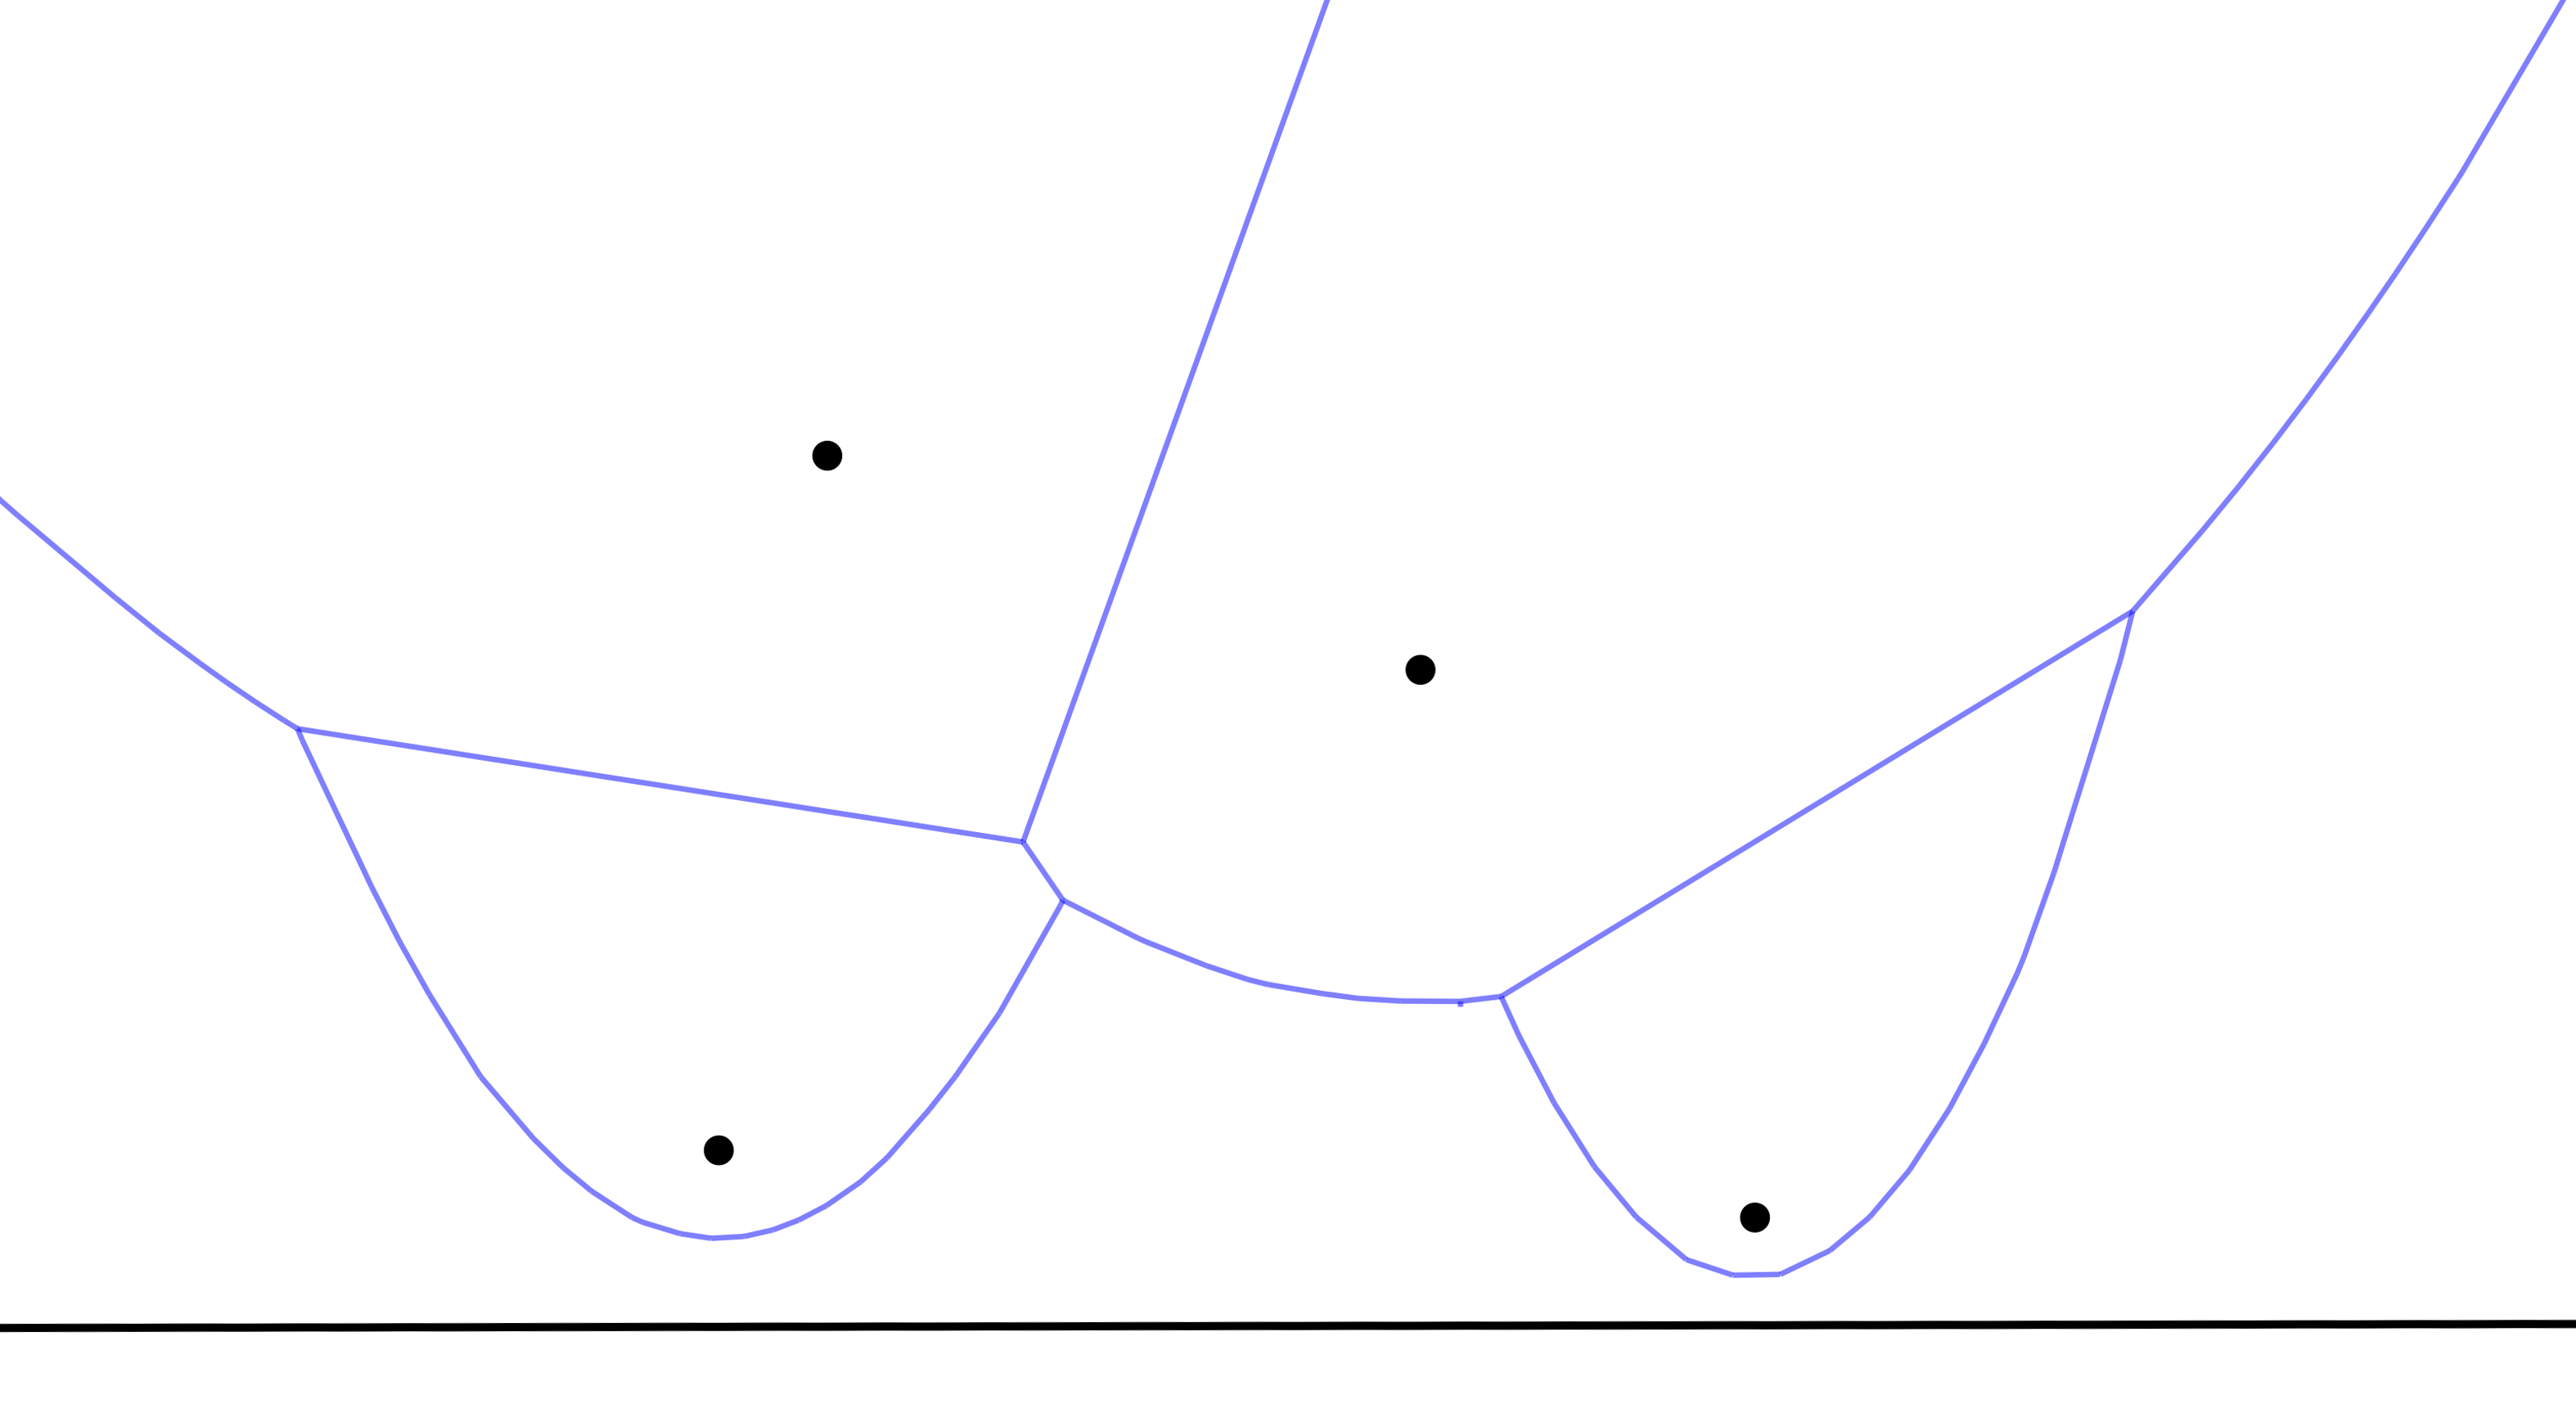
\includegraphics[scale=0.5]{../bilder/beachline.png}}
	\hspace{2cm}
	\subfloat[AVL-Baum\label{fig:beachline_tree}]
		{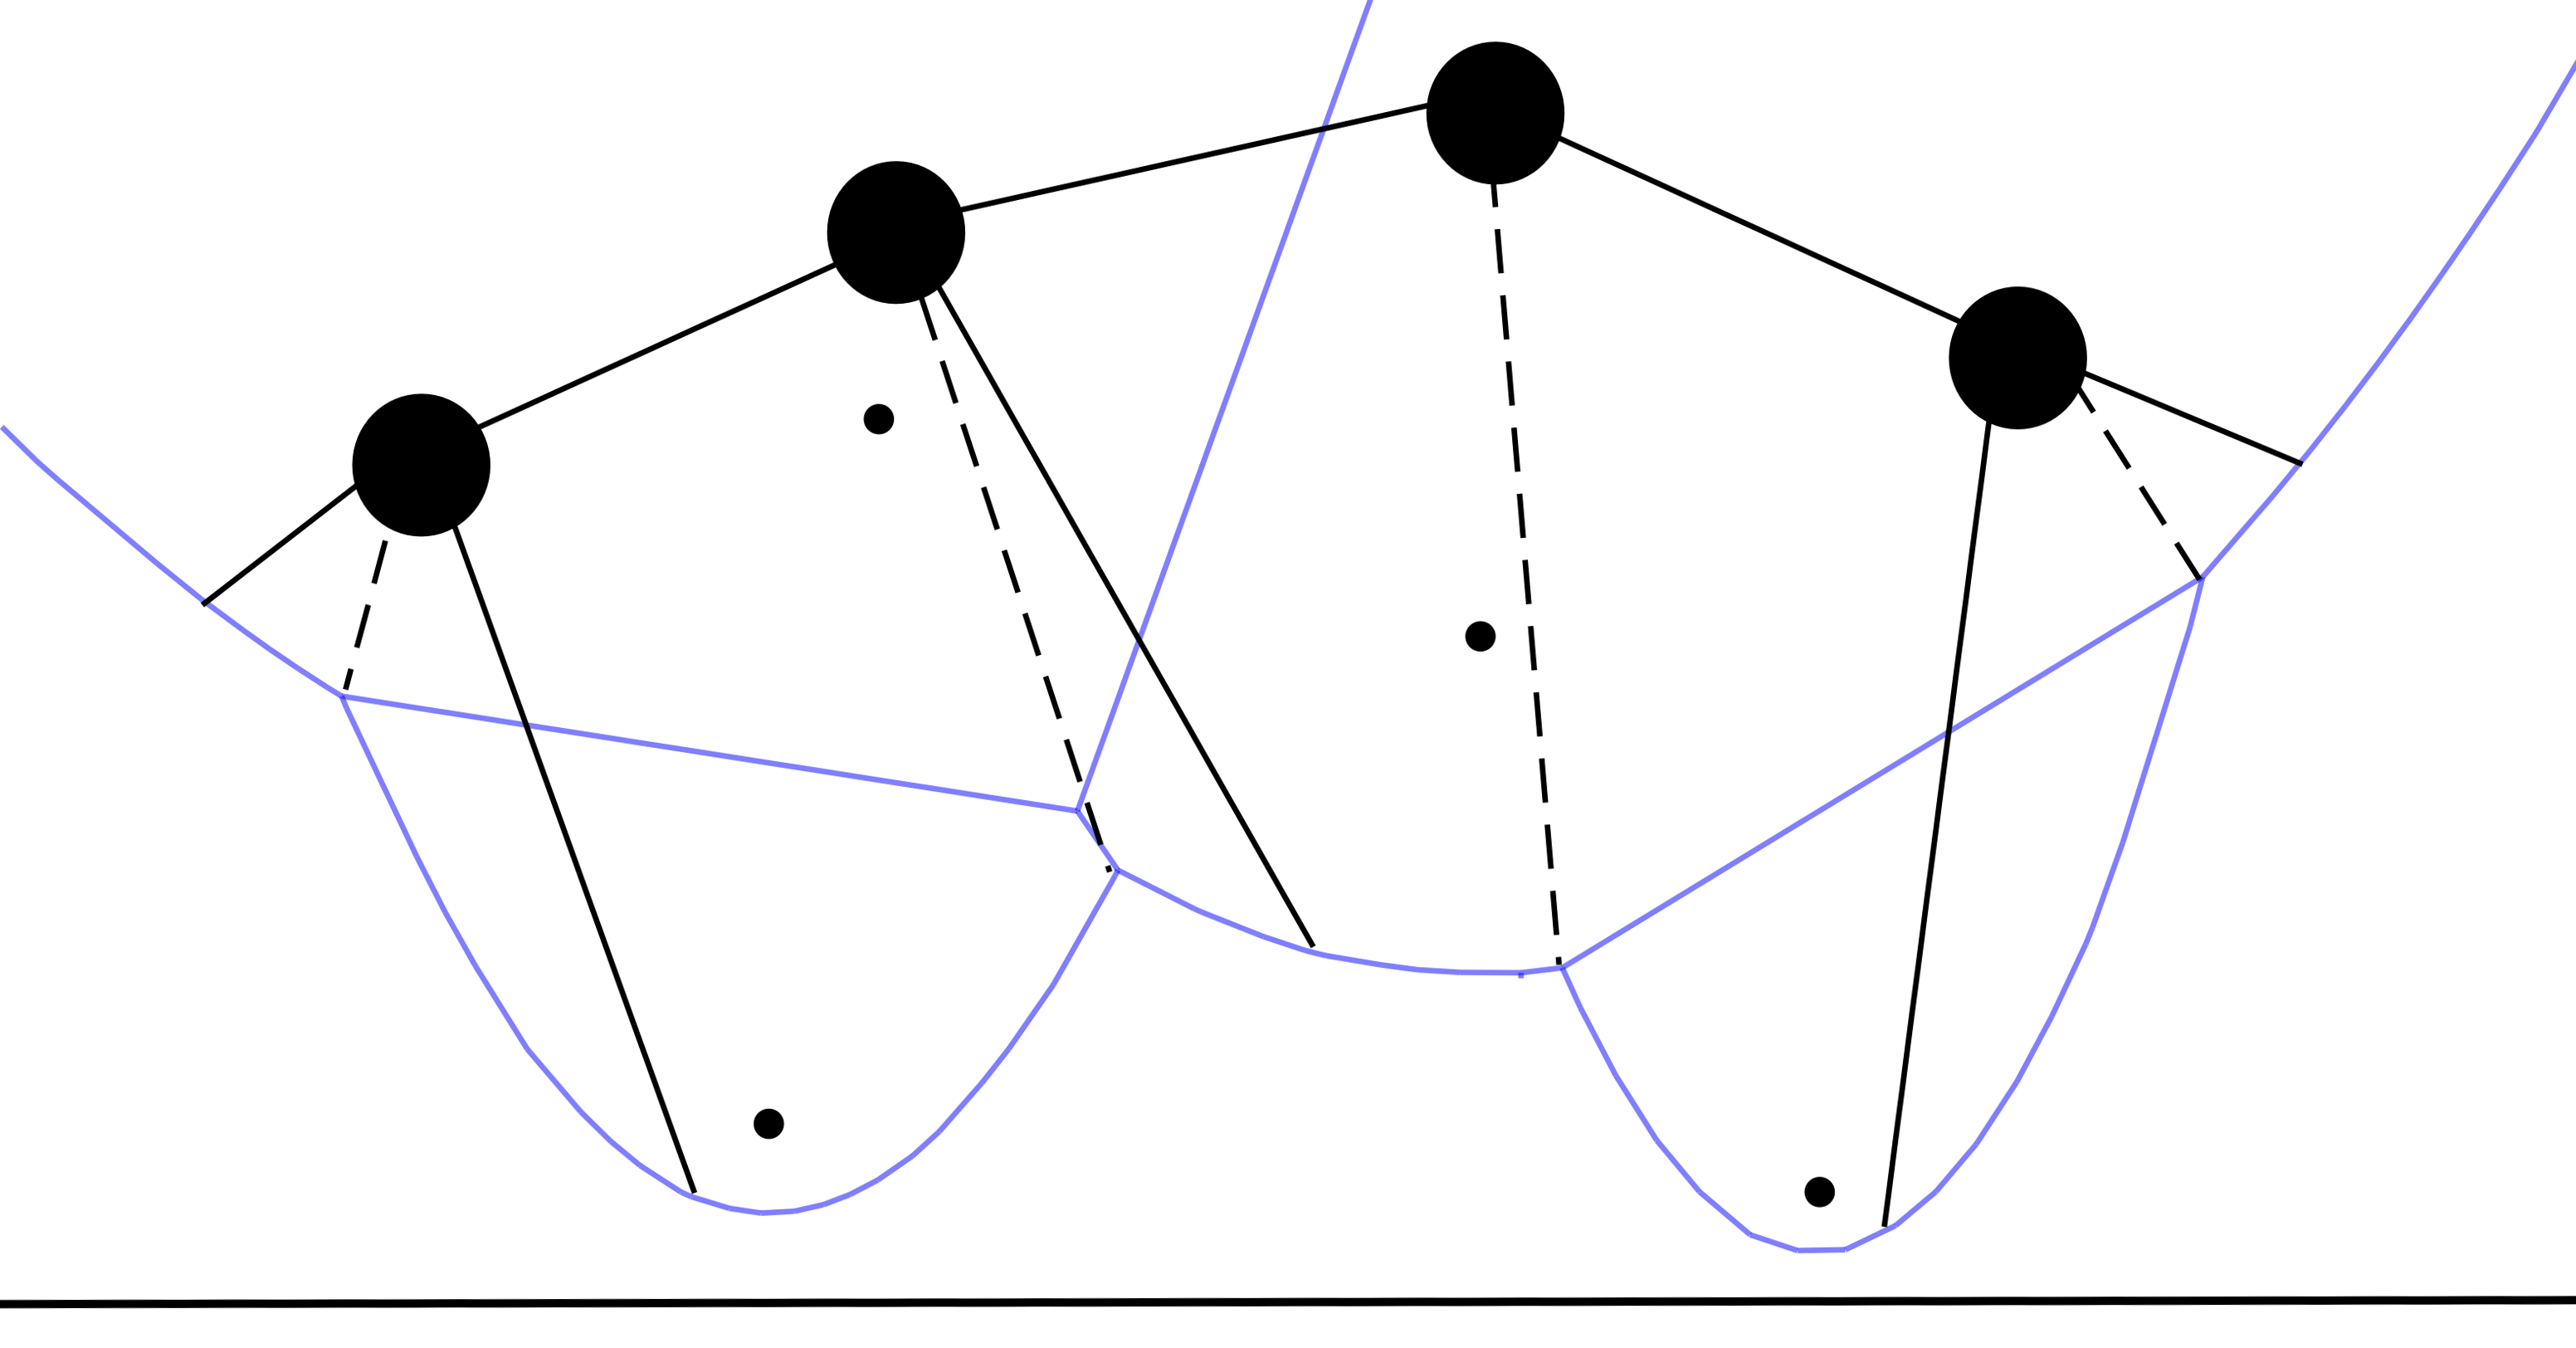
\includegraphics[scale=0.5]{../bilder/beachline_tree.png}}
	\caption{Küstenlinie und AVL-Baum für Fortunes Algorithmus}
	\label{fig:fortune}	
\end{figure}

In Abbildung~\ref{fig:fortune} wird eine Punktmenge, eine Sweep-Line, eine Küstenlinie und der AVL-Baum zur Speicherung der Küstenlinie dargestellt. Die gestrichelten Linien stellen die Zuordnung von inneren Knoten zu Schnittpunkten dar und sind keine Kanten des Baums.

Trifft die Sweep-Line auf einen Punkt aus $S$, so muss ein neuer Parabelbogen in die Küstenlinie eingefügt werden. Liegen die Punkte dreier benachbarter Parabelbögen auf einem Kreis und trifft die Sweep-Line den tiefsten Punkt dieses Kreises, so muss ein Parabelbogen sowie ein Schnittpunkt aus der Küstenlinie entfernt werden.

Einfügen und entfernen eines Knoten hat für einen AVL-Baum mit $n$ Knoten eine Zeitkomplexität von $O(\log{n})$. Für eine Punktmenge mit $n$ Punkten ergibt sich damit eine Gesamtzeitkomplexität für die Bestimmung des Minimum-Vornoi-Diagramms von $O(n \log{n})$.

\subsection*{Algorithmus von Skyum}

Skyum beschreibt in \autocite{skyum1991} einen Algorithmus, welcher aus den Punkten auf der konvexen Hülle einer Punktmenge deren Maximum-Voronoi-Diagramm bestimmt. Durch je zwei aufeinanderfolgende Punkte auf der konvexen Hülle werden die Knoten "`im Unendlichen"' bestimmt. Um die restlichen Knoten zu bestimmen, werden aus je drei aufeinanderfolgenden Punkten, $P_1,P_2,P_3$, auf der konvexen Hülle Dreiecke gebildet. Diese werden nach Umkreisradius und Winkel bei $P_2$ sortiert. Zu dem Dreieck mit maximalen Umkreisradius bzw. Winkel wird der Umkreismittelpunkt bestimmt. Der Umkreismittelpunkt ist ein Knoten. Anschließend wird $P_2$ aus der Eingabepunktmenge entfernt, wodurch sich ggf. neue Dreiecke ergeben. Es werden alle Dreiecke, an denen $P_2$ beteiligt ist, aus der Sequenz der Dreiecke entfernt. Die neuen Dreiecke werden in die sortierte Sequenz der Dreiecke eingefügt. Das Maximum-Voronoi-Diagramm ist fertig, sobald kein Dreieck mehr in der Sequenz ist.

Der Algorithmus hat für eine Punktmenge mit $n$ Punkten eine Laufzeitkomplexität von $O(n \log{n})$. Die Punkte auf der konvexen Hülle werden durch das Konturpolygonverfahren, welches in \autocite{ProPra2012} beschrieben ist, bestimmt. Dieses Verfahren hat ebenfalls eine Laufzeitkomplexität von $O(n \log{n})$ für eine Punktmenge mit $n$ Punkten.

\subsection*{Die Doppelt Verkettete Kantenliste}

Die \emph{doppelt verkettete Kantenliste}, kurz \emph{DVK}, ist ein abstrakter Datentyp zur Repräsentation von Graphen. Sie wird in \autocite{deBerg2010} beschrieben. Die DVK enthält je eine Menge für Knoten, Flächen und Halb-Kanten. Daher kann leicht über die entsprechenden Elemente iteriert werden.

Ein \emph{Knoten} enthält seine Koordinaten und eine Referenz auf eine beliebige Halb-Kante, welche den Knoten als Ursprung hat.

Eine \emph{Fläche} enthält eine Referenz auf ihre äußere Komponente und auf jede innere Komponente. Die äußere Komponente ist eine Halb-Kante, welche zur äußeren Begrenzung beiträgt und eine innere Komponente ist eine Halb-Kante, welche zur Begrenzung eines Loches in der Fläche beiträgt. Für die Speicherung von Voronoi-Zellen als Flächen, enthält die Fläche zusätzlich noch die Koordinaten des Zentrums der Voronoi-Zelle.

Eine \emph{Halb-Kante} hat eine Referenz auf ihren Ursprungsknoten, auf ihre Vorgänger-Halb-Kante, auf ihre Nachfolger-Halb-Kante, auf eine Fläche, zu deren Kantenmenge sie gehört, und auf ihre Zwillings-Halb-Kante. Die Kombination aus Halb-Kante und Zwilling wird im Folgenden einfach als \emph{Kante} bezeichnet.


\begin{figure}[htbp]
	\centering
	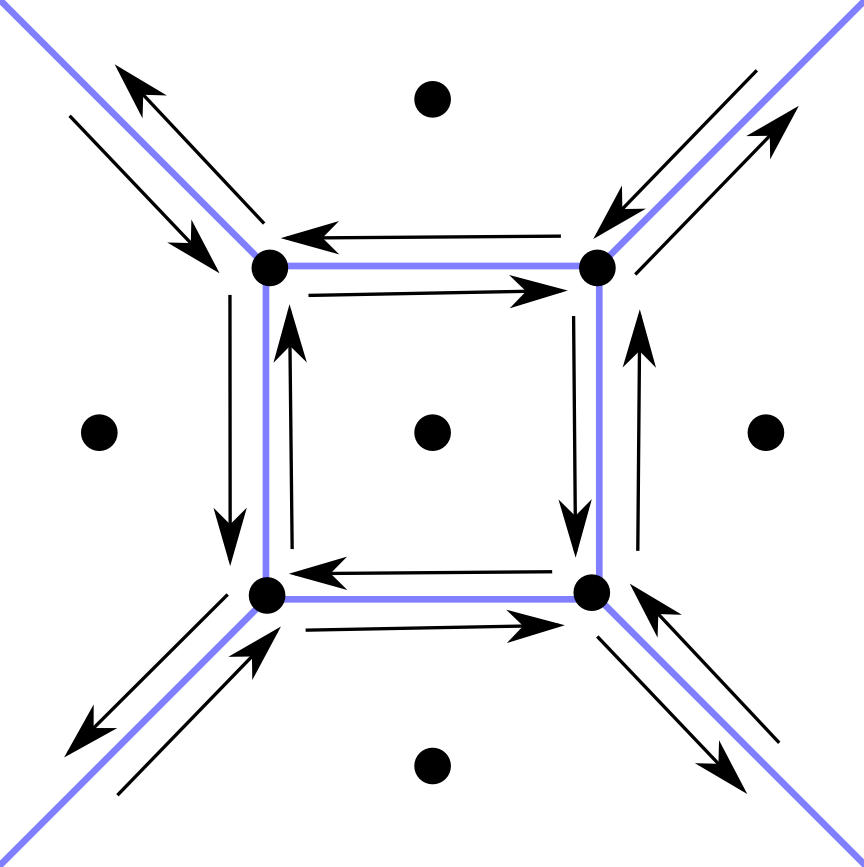
\includegraphics[scale=1.0]{../bilder/voronoi_min_dcel.png}
	\caption{DVK eines Minimum-Voronoi-Diagramms}
	\label{fig:voronoi_min_dcel}
\end{figure}

In Abbildung~\ref{fig:voronoi_min_dcel} ist die DVK eines Minimum-Voronoi-Diagramms dargestellt. Die Halb-Kanten liegen in den von ihnen begrenzten Flächen und sind im Uhrzeigersinn verkettet. Der Zwilling jeder Halb-Kante liegt in einer benachbarten Fläche bzw. Voronoi-Zelle. Knoten des Diagramms und die Zentren der Flächen sind als schwarze Punkte dargestellt.

\section{Ein Algorithmus zur Bestimmung der Shape-Spektren}

Vor der Beschreibung des Algorithmus werden wichtige Teilschritte erklärt und es wird auf den Umgang mit unendlich langen Kanten im Voronoi-Diagramm eingegangen.

\subsection*{Bestimmung eines Knotens des Delaunay-Graphen aus der DVK eines Voronoi-Diagramms}

Ein Knoten des Delaunay-Graphen und die Grenzen seines Shape-Spektrums können aus einer Flächen $f(P)$ der DVK eines Voronoi-Diagramms bestimmt werden. Jedes Zentrum $P$ einer Fläche ist auch ein Knoten des Delaunay-Graphen und umgekehrt. Um das Shape-Spektrum des Knotens zu bestimmen muss der Abstand von $P$ zu allen Vorgänger- und Nachfolger-Kanten der äußeren Komponente der Fläche bestimmt werden. Sei nun $d_{\min}(f(P))$ der minimale und $d_{\max}(f(P))$ der maximale dieser Abstände.

\subsection*{Bestimmung einer Kante des Delaunay-Graphen aus der DVK eines Voronoi-Diagramms}

Eine Kante des Delaunay-Graphen und die Grenzen seines Shape-Spektrums können aus einer Kante $b$ der DVK eines Voronoi-Diagramms bestimmt werden. Jeder Kante $b$ des Voronoi-Diagramms ist eine eindeutige duale Kante $e$ des Delaunay-Graphen zugeordnet und umgekehrt. Anfangs- und Endpunkt von $e$ sind die Zentren derjenigen Flächen, welche durch $b$ getrennt werden. Um das Shape-Spektrum der Kante $e$ zu bestimmen muss der minimale und der maximale Abstand eines Endpunkts von $e$ zu $b$ bestimmt werden. Sei nun $d_{\min}(e,b)$ der minimale und $d_{\max}(e,b)$ der maximale Abstand.

\subsection*{Eine untere Schranke für unendliche Abstände im Voronoi-Diagramm}

In einem Voronoi-Diagramm können Kanten vorkommen, welche Strahlen oder Geraden sind. Diese Kanten werden für die praktische Berechnung durch Strecken angenähert. Die Länge dieser Strecken muss größer sein als der maximal vorkommende Abstand eines Zentrums einer abgeschlossenen Voronoi-Zelle zu ihrem Rand. Dieser Wert wird durch die Konstante \emph{BIGVAL} repräsentiert. Alle Abstände im Voronoi-Diagramm, welche größer sind als dieser Wert, gelten als unendlich. Der Wert von \emph{BIGVAL} ist abhängig von den Koordinaten der Eingabepunktmenge und muss an diese angepasst werden. Für praktische Anwendungen wurde das zehnfache des maximal zu erwartenden Abstands zweier Punkte verwendet. Wird zur Eingabe einer Punktmenge eine rechteckige Zeichenfläche verwendet wird, so ist der maximale Abstand zweier Punkte gleich der Diagonalen dieser Zeichenfläche.

\subsection*{Der Algorithmus}

Die Eingabe des Algorithmus zur Bestimmung der Shape-Spektren ist eine Punktmenge $S$. Seine Ausgabe ist die Menge der positiven Shape-Spektren der Knoten und Kanten des Minimum-Delaunay-Graphen von $S$, $PV(S)$ und $PE(S)$, die Menge der negativen Shape-Spektren der Knoten und Kanten des Maximum-Delaunay-Graphen von $S$, $NV(S)$ und $NE(S)$, sowie die positiven und negativen Shape-Schwellen der Punktmenge, $Bd^+(S)$ und $Bd^-(S)$. Aus Gründen der Übersichtlichkeit ist der Algorithmus in einen Algorithmus zur Bestimmung der positiven Shape-Spektren (Algorithmus~\ref{alg:posSpec}) und einen Algorithmus zur Bestimmung der negativen Shape-Spektren (Algorithmus~\ref{alg:negSpec}) aufgeteilt worden.

\begin{algorithm}\caption{Bestimmung der positiven Shape-Spektren}\label{alg:posSpec}
\begin{algorithmic}[0]
\Function{PositiveShapeSpektren}{$S$}
	\State $PV(S) \gets \oslash$
	\State $PE(S) \gets \oslash$
	\State $Bd^+(S) \gets \oslash$
	\State Bestimme DVK von $VD_{\min}(S)$
	\ForAll{$f(P) \in VD_{\min}(S)$}
		\If{$d_{\max}(f(P)) < \text{ BIGVAL}$}
			\State $Sp^+(P) \gets (0, d_{\max}(f(P))]$
			\State $Bd^+(S) \gets Bd^+(S) \cup \lbrace d_{\max}(f(P)) \rbrace$
		\Else
			\State $Sp^+(P) \gets (0, \infty)$
		\EndIf
		\State $PV(S) \gets PV(S) \cup \lbrace Sp^+(P) \rbrace$
	\EndFor
	\ForAll{$b \in VD_{\min}(S)$}
		\State Bestimme duale Delaunay-Kante $e$ zu $b$
		\State $Bd^+(S) \gets Bd^+(S) \cup \lbrace d_{\min}(e,b) \rbrace$
		\If{$d_{\max}(e,b) < \text{ BIGVAL}$}
			\State $Sp^+(e) \gets [d_{\min}(e,b),d_{\max}(e,b)]$
			\State $Bd^+(S) \gets Bd^+(S) \cup \lbrace d_{\max}(e,b) \rbrace$
		\Else
			\State $Sp^+(e) \gets [d_{\min}(e,b),\infty)$
		\EndIf
		\State $PE(S) \gets PE(S) \cup \lbrace Sp^+(e) \rbrace$
	\EndFor
	\State \textbf{return} $(PV(S),PE(S),Bd^+(S))$
\EndFunction
\end{algorithmic}
\end{algorithm}

\begin{algorithm}\caption{Bestimmung der negative Shape-Spektren}\label{alg:negSpec}
\begin{algorithmic}[0]
\Function{NegativeShapeSpektren}{$S$}
	\State $NV(S) \gets \oslash$
	\State $NE(S) \gets \oslash$
	\State $Bd^-(S) \gets \oslash$
	\State Bestimme DVK von $VD_{\max}(S)$
	\ForAll{$f(P) \in VD_{\max}(S)$}
		\State $Sp^-(P) \gets (-\infty,-d_{\min}(f(P))]$
		\State $Bd^-(S) \gets Bd^-(S) \cup \lbrace -d_{\min}(f(P)) \rbrace$
		\State $NV(S) \gets NV(S) \cup \lbrace Sp^-(P) \rbrace$
	\EndFor
	\ForAll{$b \in VD_{\max}(S)$}
		\State Bestimme duale Delaunay-Kante $e$ zu $b$
		\State $Bd^-(S) \gets Bd^-(S) \cup \lbrace d_{\min}(e,b) \rbrace$
		\If{$d_{\max} < \text{ BIGVAL}$}
			\State $Sp^-(e) \gets [-d_{\max}(e,b),-d_{\min}(e,b)]$
			\State $Bd^-(S) \gets Bd^-(S) \cup \lbrace -d_{\max} \rbrace$
		\Else
			\State $Sp^-(e) \gets (-\infty,-d_{\min}(e,b)]$
		\EndIf
		\State $NE(S) \gets NE(S) \cup \lbrace Sp^-(e) \rbrace$
	\EndFor
	\State \textbf{return} $(NV(S),NE(S),Bd^-(S))$
\EndFunction
\end{algorithmic}
\end{algorithm}

\begin{lemma}\label{lemma:shape_compl}
Die Zeitkomplexität für die Bestimmung der Shape-Spektren bezüglich der Größe $n$ der Punktmenge $S$ ist $O(n \log{n})$.
\end{lemma}

\begin{proof}[Beweis zu Lemma \ref{lemma:shape_compl}]
Die Algorithmen zur Berechnung der Voronoi-Diagramme von $S$ haben eine Zeitkomplexität von $O(n \log{n})$. Die Anzahl der Zellen und Kanten im Voronoi-Diagramm ist linear zu $n$. Es wird ein Shape-Spektrum pro Kante und ein Shape-Spektrum pro Zentrum je mit konstanter Zeitkomplexität berechnet. Damit ist die Zeitkomplexität der Berechnung aller Kanten- und Knoten-Shape-Spektren linear zu $n$.
\end{proof}

\section[Ein Algorithmus zur Konstruktion der $\alpha$-Shape]{Ein Algorithmus zur Konstruktion der \boldmath{$\alpha$}-Shape}

Die Eingabe des Algorithmus zur Bestimmung der $\alpha$-Shape (Algorithmus~\ref{alg:shape}) ist der Parameter $\alpha$, die Menge der positiven Shape-Spektren der Knoten und Kanten des Minimum-Delaunay-Graphen von $S$, $PV(S)$ und $PE(S)$, sowie die Menge der negativen Shape-Spektren der Knoten und Kanten des Maximum-Delaunay-Graphen von $S$, $NV(S)$ und $NE(S)$. Seine Ausgabe ist die Menge der Knoten der $\alpha$-Shape von $S$, $AV(S,\alpha)$, und die Menge der Kanten der $\alpha$-Shape von $S$, $AE(S,\alpha)$.

\begin{algorithm}\caption{Bestimmung der $\alpha$-Shape}\label{alg:shape}
\begin{algorithmic}[0]
\Function{AlphaShape}{$\alpha,PV(S),PE(S),NV(S),NE(S)$}
	\State $AV(S,\alpha) \gets \oslash$
	\State $AE(S,\alpha) \gets \oslash$
	\If{$\alpha > 0$}
		\ForAll{$Sp^+(P) \in PV(S)$}
			\If{$\alpha \in Sp^+(P)$}
				$AV(S,\alpha) \gets AV(S,\alpha) \cup \lbrace P \rbrace$
			\EndIf
		\EndFor
		\ForAll{$Sp^+(e) \in PE(S)$}
			\If{$\alpha \in Sp^+(e)$}
				$AE(S,\alpha) \gets AE(S,\alpha) \cup \lbrace e \rbrace$
			\EndIf
		\EndFor
	\ElsIf{$\alpha < 0$}
		\ForAll{$Sp^-(P) \in NV(S)$}
			\If{$\alpha \in Sp^-(P)$}
				$AV(S,\alpha) \gets AV(S,\alpha) \cup \lbrace P \rbrace$
			\EndIf
		\EndFor
		\ForAll{$Sp^-(e) \in PE(S)$}
			\If{$\alpha \in Sp^-(e)$}
				$AE(S,\alpha) \gets AE(S,\alpha) \cup \lbrace e \rbrace$
			\EndIf
		\EndFor
	\EndIf	
	\State \textbf{return} $(AV(S,\alpha),AE(S,\alpha))$
\EndFunction
\end{algorithmic}
\end{algorithm}

\begin{lemma}\label{lemma:alpha_compl}
Die Zeitkomplexität für die Bestimmung der $\alpha$-Shape aus Shape-Spektren bezüglich der Größe $n$ der Punktmenge $S$ ist linear.
\end{lemma}

\begin{proof}[Beweis zu Lemma \ref{lemma:alpha_compl}]
Die Mächtigkeit der Mengen der Shape-Spektren verhält sich linear zu $n$.
\end{proof}

\section{Shape-Spektrum-Algorithmen}

Mit Hilfe von Shape-Spektren lassen sich auch noch andere interessante Eigenschaften von Punktmengen bestimmen.

\subsection*{Das dichteste Paar}
Der Abstand des dichtesten Paares einer Punktmenge $S$ ist das doppelte des kleinsten Wertes in $Bd^+(S)$. Das dichteste Paar selbst lässt sich bestimmen, indem man in der Menge $PE(S)$ dasjenige $Sp^+(e)$ mit $e=(P_1,P_2)$ sucht, dessen untere Schranke gleich dem kleinsten positiven Wert ist. Das dichteste Paar ist dann $(P_1,P_2)$.

\subsection*{Der kleinste einschließende Kreis}
Der Radius $r$ des kleinsten einschließenden Kreises einer Punktmenge $S$ ist der kleinste Betrag in $Bd^-(S)$. Der Mittelpunkt des kleinsten einschließenden Kreises lässt sich folgendermaßen bestimmen: Man sucht in der Menge $NE(S)$ diejenigen $Sp^-(e)$, deren obere Schranke gleich der Negation von $r$ ist. Existiert nur ein solches $Sp^-(e)$, so ist der Mittelpunkt von $e$ auch der Mittelpunkt des kleinsten Kreises. Existieren mehrere solche $Sp^-(e)$, so bilden die Kanten $e$ ein Polygon, dessen Umkreis-Mittelpunkt der Mittelpunkt des kleinsten einschließenden Kreises ist.

\subsection*{Der Rand der konvexen Hülle}
Die konvexe Hülle lässt sich folgendermaßen bestimmen: Suche in der Menge $PE(S)$ diejenigen $Sp^+(e)$, deren obere Schranke gleich $\infty$ ist. Alternativ kann man auch in der Menge $NE(S)$ nach denjenigen $Sp^-(e)$ suchen, deren untere Schranke gleich $-\infty$ ist. Der Rand der konvexen Hülle ist gleich der Menge der Kanten $e$.
